\documentclass[a4paper,oneside,12pt]{article}
\usepackage[utf8]{inputenc}
\usepackage[czech]{babel}
\usepackage[pdftex]{graphicx}
\usepackage{mathtools}
\addtolength{\textwidth}{2cm}
\addtolength{\hoffset}{-1cm}
\addtolength{\textheight}{5cm}
\addtolength{\voffset}{-2.5cm}

\author{Matej Soroka (xsorok02)}
\date{\today}
\title{Projekt z predmetu IEL}

\begin{document}
	\maketitle
	\newpage

	\tableofcontents
	\newpage

	\section{Riesenie 2017/18}
	\maketitle

	\subsection{Příklad 1}

	Stanovte napětí $U_{R1}$ a proud $I_{R1}$. Použijte metodu postupného
	zjednodušování obvodu.

	\begin{table}[h]
		\begin{center}
			\begin{tabular}{|c|c|c|c|c|c|c|c|c|c|c|}
				\hline
				sk. & $U_{1}$ [$V$] & $U_{2}$ [$V$] & $R_{1}$ [$\Omega$] & $R_{2}$ [$\Omega$] & $R_{3}$ [$\Omega$] & $R_{4}$ [$\Omega$] & $R_{5}$ [$\Omega$] & $R_{6}$ [$\Omega$] & $R_{7}$ [$\Omega$] & $R_{8}$ [$\Omega$] \\
				\hline
				D & 105 & 85 & 420 & 980 & 330 & 280 & 310 & 710 & 240 & 200 \\
				\hline
			\end{tabular}
		\end{center}
	\end{table}

	\begin{figure}[h]
		\begin{center}
			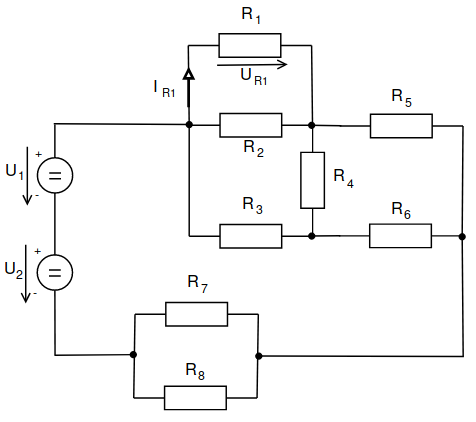
\includegraphics[width=8cm,keepaspectratio]{img/pr1.png}
		\end{center}
	\end{figure}

	Zapojení postupně zjednodušíme:
	\begin{eqnarray*}
		U &= & U_{1} + U_{2} = 105 + 85 = 190V\\
		R_{12} &= & R_{1} || R_{2} = \frac{R_{1} * R_{2}}{R_{1} + R_{2}} = \frac{420 * 980}{420 + 980} = 294 \Omega\\
		R_{78} &= & R_{7} || R_{8} = \frac{R_{7} * R_{8}}{R_{7} + R_{8}} = \frac{240 * 200}{240 + 200} = 109.0909 \Omega\\
	\end{eqnarray*}

	Vzniklý trojúhelník [$R_{4}$, $R_{5}$, $R_{6}$] převedeme na hvězdu:
	\begin{eqnarray*}
		R_{a} &= & \frac{R_{4} * R_{5}}{R_{4} + R_{5} + R_{6}} = \frac{280 * 310}{280 + 310 + 710} = 66.7692 \Omega\\
		R_{b} &= & \frac{R_{4} * R_{6}}{R_{4} + R_{5} + R_{6}} = \frac{280 * 710}{280 + 310 + 710} = 152.9231 \Omega\\
		R_{c} &= & \frac{R_{5} * R_{6}}{R_{4} + R_{5} + R_{6}} = \frac{310 * 710}{280 + 310 + 710} = 169.3077 \Omega\\
	\end{eqnarray*}

	Dále zjednodušíme:
	\begin{eqnarray*}
		R_{12a} &= & R_{12} + R_{a} = 294 + 66.7692 = 360.7692 \Omega\\
		R_{3b} &= & R_{3} + R_{b} = 330 + 152.9231 = 482.9231 \Omega\\
		R_{123ab} &= & \frac{R_{12a} * R_{3b}}{R_{12a} + R_{3b}} = \frac{360.7692 * 482.9231}{360.7692 + 482.9231} = 206.5016 \Omega\\
	\end{eqnarray*}

	Vypočítame ekvivalentný odpor
	\begin{eqnarray*}
		R_{EKV} &= & R_{123ab} + R_{78} + R_{c} = 206.5016 + 109.0909 + 169.3077 = 484.9002 \Omega\\
	\end{eqnarray*}

	Vypočteme proud zdroje:
	\begin{eqnarray*}
		I &= & \frac{U}{R_{EKV}} = \frac{190}{484.9002} = 0.3918 A\\
	\end{eqnarray*}

	Ze získaných hodnot vypočteme hledané hodnoty $I_{R1}$ a $U_{R1}$:
	\begin{eqnarray*}
		U_{123ab} &= & I * R_{123ab} = 0.3918 * 206.50157 = 80.9142V\\
		I_{12a} &= &\frac{U_{123ab}}{R_{12a}} = \frac{80.9142}{360.7692} = 0.2243A\\
		U_{R12} &= & I_{12a} * R_{12} = 0.2243 * 294 = 65.9390V\\
l		I_{R1} &= &\frac{U_{R12}}{R_{1}} = \frac{65.9390V}{420} = 0.1570A\\
		U_{R1} &= & I_{R1} * R_{1} = 0.1570 * 420 = 65.9390V\\
	\end{eqnarray*}

	Hledané hodnoty $I_{R3}$ a $U_{R3}$ jsou:
	\begin{eqnarray*}
		I_{R1} &= & 0.1570A\\
		U_{R1} &= & 65.9390V\\
	\end{eqnarray*}

	\newpage

	\subsection{Příklad 2}

	Stanovte napětí $U_{R3}$ a proud $I_{R3}$. Použijte metodu Théveninovy věty.

	\begin{table}[h]
		\begin{center}
			\begin{tabular}{|c|c|c|c|c|c|c|}
				\hline
				sk. & $U_{1}$ [$V$] & $U_{2}$ [$V$] & $R_{1}$ [$\Omega$] & $R_{2}$ [$\Omega$] & $R_{3}$ [$\Omega$] & $R_{4}$ [$\Omega$]\\
				\hline
				G & 180 & 250 & 315 & 615 & 180 & 460 \\
				\hline
			\end{tabular}
		\end{center}
	\end{table}

	\begin{figure}[h]
		\begin{center}
			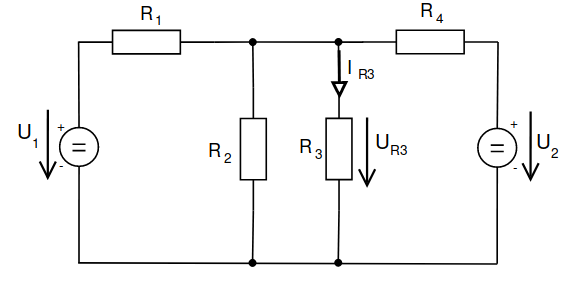
\includegraphics[width=8cm,keepaspectratio]{img/pr2.png}
		\end{center}
	\end{figure}

	Zjednotíme vnútorné odpory paralelne a vypočítame $R_{i}$:
	\begin{eqnarray*}
		R_{23} &= & R_{2} || R_{3} = \frac{R_{2} * R_{3}}{R_{2} + R_{3}} = \frac{615 * 180}{615 + 180} = 139.2453 \Omega\\
		R_{i} &= & R_{1} || R_{4} = \frac{R_{1} * R_{4}}{R_{1} + R_{4}} = \frac{315 * 460}{315 + 460} = 186.9677 \Omega\\
	\end{eqnarray*}

	Vypocitame prud $I_{x}$ tecuci obvodom bez odporu $R_{23}$ a napatie $U_{i}$:
	\begin{eqnarray*}
		I_{x} &= & \frac{U_{2} - U_{1}}{R_{1} + R_{4}} = \frac{250 - 180}{315 + 460} = 0.0903 A\\
	\end{eqnarray*}

	Dle II. Kirchhoffova zákona vypočteme napětí $U_{i}$ ze smyčky tvořené větvemi s rezistory $R_{1}$, $R_{2}$ a $R_{3}$:
	\begin{eqnarray*}
		U_{i} &= & U_{2} - R_{4} * I_{x} \\
		U_{i} &= & 250 - 460 * 0.0903 \\
		U_{i} &= & 208.4516V \\
	\end{eqnarray*}

	Ze získaných hodnot vypočteme hledané hodnoty $I_{R23}$ a $U_{R23}$:
	\begin{eqnarray*}
		I_{R23} &= & \frac{U_{i}}{R_{i} + R_{23}} = \frac{208.4516}{186.9677 + 139.2453} = 0.6390 A\\
		U_{R23} &= & R_{23} * I_{R23} = 139.2453 * 0.6390 = 88.9784 V\\
	\end{eqnarray*}

	Ziskali sme prud a napatie pre zjednoduseny rezistor $R_{23}$ z ktoreho vypocitame $I_{R3}$ a $U_{R3}$:
	\begin{eqnarray*}
		I_{R3} &= & \frac{R_{2}}{R_{2} + R_{3}} * I_{R23} = \frac{615}{615 + 180} * 0.6390 = 0.4943 A\\
		U_{R3} &= & R_{3} * I_{R3} = 180 * 0.4943 = 88.9784 V\\
	\end{eqnarray*}

	Hledané hodnoty $I_{R3}$ a $U_{R3}$ jsou:
	\begin{eqnarray*}
		I_{R3} &= & 0.4943 A\\
		U_{R3} &= & 88.9784 V\\
	\end{eqnarray*}

	\newpage

	\subsection{Příklad 3}

	Stanovte napětí $U_{R5}$ a proud $I_{R5}$. Použijte metodu uzlových napětí ($U_{A}$, $U_{B}$, $U_{C}$).
	
	\begin{table}[h]
		\begin{center}
			\begin{tabular}{|c|c|c|c|c|c|c|}
				\hline
				sk. & $U_{1}$ [$V$] & $U_{2}$ [$V$] & $R_{1}$ [$\Omega$] & $R_{2}$ [$\Omega$] & $R_{3}$ [$\Omega$] & $R_{4}$ [$\Omega$]\\
				\hline
				G & 180 & 250 & 315 & 615 & 180 & 460 \\
				\hline
			\end{tabular}
		\end{center}
	\end{table}

	\begin{figure}[h]
		\begin{center}
			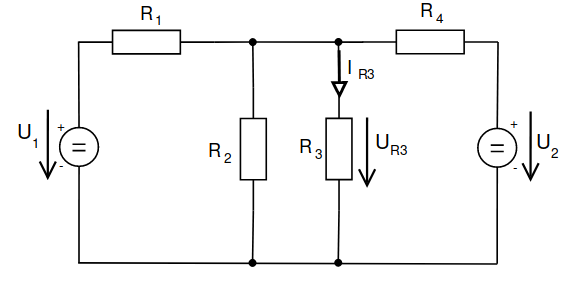
\includegraphics[width=8cm,keepaspectratio]{img/pr2.png}
		\end{center}
	\end{figure}

	Zjednotíme vnútorné odpory paralelne a vypočítame $R_{i}$:
	\begin{eqnarray*}
		R_{23} &= & R_{2} || R_{3} = \frac{R_{2} * R_{3}}{R_{2} + R_{3}} = \frac{615 * 180}{615 + 180} = 139.2453 \Omega\\
		R_{i} &= & R_{1} || R_{4} = \frac{R_{1} * R_{4}}{R_{1} + R_{4}} = \frac{315 * 460}{315 + 460} = 186.9677 \Omega\\
	\end{eqnarray*}

	Vypocitame prud $I_{x}$ tecuci obvodom bez odporu $R_{23}$ a napatie $U_{i}$:
	\begin{eqnarray*}
		I_{x} &= & \frac{U_{2} - U_{1}}{R_{1} + R_{4}} = \frac{250 - 180}{315 + 460} = 0.0903 A\\
	\end{eqnarray*}

	Dle II. Kirchhoffova zákona vypočteme napětí $U_{i}$ ze smyčky tvořené větvemi s rezistory $R_{1}$, $R_{2}$ a $R_{3}$:
	\begin{eqnarray*}
		U_{i} &= & U_{2} - R_{4} * I_{x} \\
		U_{i} &= & 250 - 460 * 0.0903 \\
		U_{i} &= & 208.4516V \\
	\end{eqnarray*}

	Ze získaných hodnot vypočteme hledané hodnoty $I_{R23}$ a $U_{R23}$:
	\begin{eqnarray*}
		I_{R23} &= & \frac{U_{i}}{R_{i} + R_{23}} = \frac{208.4516}{186.9677 + 139.2453} = 0.6390 A\\
		U_{R23} &= & R_{23} * I_{R23} = 139.2453 * 0.6390 = 88.9784 V\\
	\end{eqnarray*}

	Ziskali sme prud a napatie pre zjednoduseny rezistor $R_{23}$ z ktoreho vypocitame $I_{R3}$ a $U_{R3}$:
	\begin{eqnarray*}
		I_{R3} &= & \frac{R_{2}}{R_{2} + R_{3}} * I_{R23} = \frac{615}{615 + 180} * 0.6390 = 0.4943 A\\
		U_{R3} &= & R_{3} * I_{R3} = 180 * 0.4943 = 88.9784 V\\
	\end{eqnarray*}

	Hledané hodnoty $I_{R3}$ a $U_{R3}$ jsou:
	\begin{eqnarray*}
		I_{R3} &= & 0.4943 A\\
		U_{R3} &= & 88.9784 V\\
	\end{eqnarray*}

	\newpage
\end{document}
